%!TEX root = 0卒業論文.tex
\clearpage

\section{\rm 教材の使用方法}

\subsection{学習方法}
授業で教員や児童がパソコン又はiPadを用いて本サイトを使用してもらうことを想定する.
本サイトの,トップページ部,Scratch 使い方の画面を参照し,Scratchの基本動作を学んでもらう.
授業内では問題画面を児童に見ていただき,問題画面,表示される制作課題のアニメーションと同じ動きになるものをScratchを用いて作成する.
作成した後に,「解説を見る」ボタンを押し,解答例,解説を読み理解してもらう流れになる.
また,スクラッチファイルをダウンロードすることが可能になっているため,自身で動作を確認することができる.
\begin{figure}[h]
\begin{center}
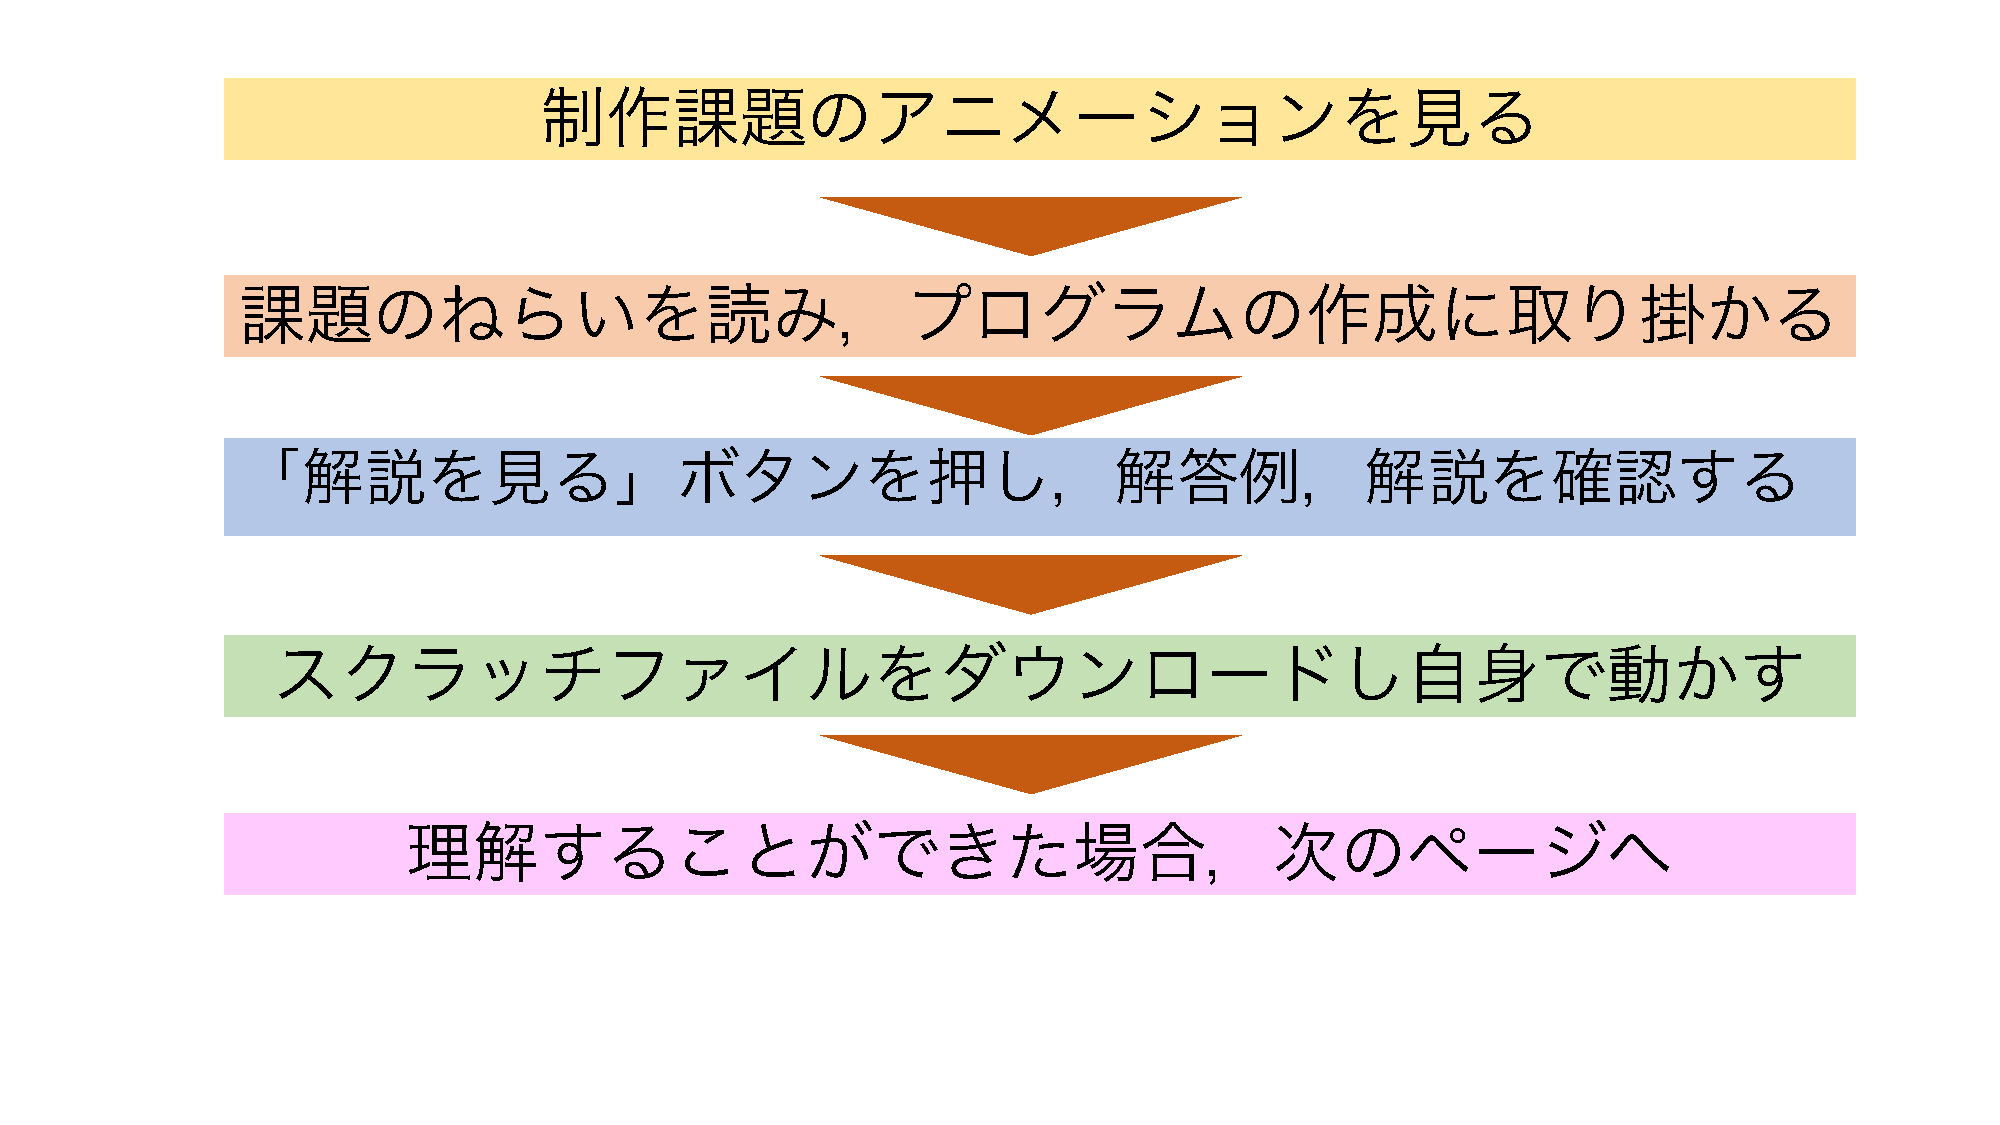
\includegraphics[width=15cm]{gakushuu.pdf}
\caption{学習方法 流れ}
\label{fig:houhou}
\end{center}
\end{figure}
